
\subsection{The Theory of Hurricanes}
\label{sec:hurr-theory}
\subsubsection{The Carnot cyclone}
\label{sec:carnot}

The hurricane can be idealised as a Carnot cycle as in Figure~\ref{fig:hurricane-carnot},
as was originally proposed by Kerry Emanuel.

\begin{figure}
\centering
    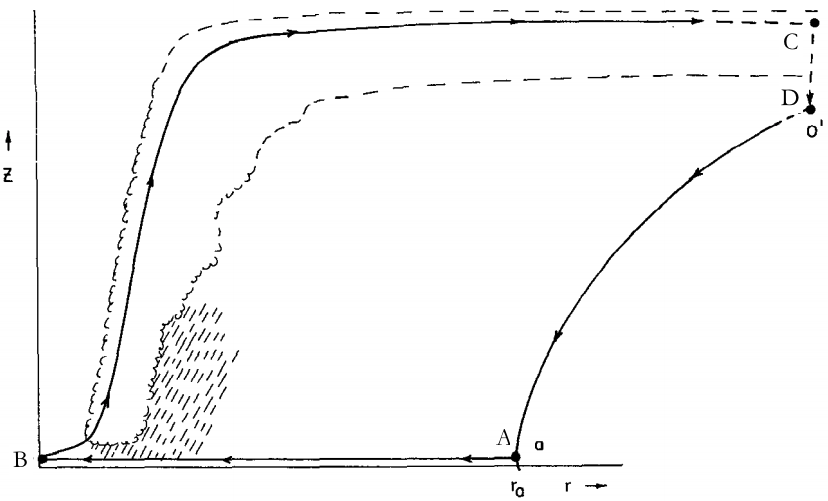
\includegraphics[width=\linewidth]{images/hurricane-carnot.png}\\
    \textit{Figure 1 from~\cite{emanuel1991theory}. }
    \caption{An idealised Carnot cycle where air parcels travel clockwise;
            travelling inwards into the eye-wall extracting thermal energy
            from the sea; adiabatically thrust up into the stratosphere
            at the eye-wall; isothermally transported out. }
            \label{fig:hurricane-carnot}

\end{figure}

The temperature of the sea surface temperature controls the hurricane.

A western boundary current has a thicker

\begin{itemize}
\item thermodynamic disequilibrium
\item cyclogenesis
\item Carnot cycle $\implies$ potential intensity limits.
\item reasons for not reaching potential intensity.
\item super-intensity cyclones.
\item weaknesses.
\end{itemize}

\subsubsection{Potential Intensity}
\label{sec:potential_intensity}

Therefore given the sea surface temperature, there is some maximum intensity
that a hurricane could reach given the rest of the climate.

This makes some simplifying assumptions, the sea is not all at the temperature
of the surface, instead only up to some depth. The depth of warm water
is larger at the western boundary currents, which means that if a hurricane
travels down the axis of the current it can reach a higher intensity than
if it does not.

\subsubsection{Cyclogenesis}
Warm air rises in cumulonimbus clouds,
 dries, and then falls down very dry.
A decrease in humidity with altitude.
 Middle level dryness.
cumulonimbus clouds clump together.
 More updrafts give more rain.

Nascent cloud cluster dies away.

Fig 14.6 compares 3 computer models.

Middle atmosphere becomes humidified.

William grey cyclogenesis~\cite{gray1975tropical}.

African Easterly Waves.

Ordinary cold front that penetrates tropics.

Tropical cyclogenesis is one of the
 great mysteries of the tropical atmosphere.

An EC does not need anything to trigger it.

Notes from Emmanuel~\cite{emanuel2005divine}.

